% FIG ch07-02 relation-number overlay (language-neutral)
\makeatletter
\@ifundefined{chsevenrelmark}{%
\newcommand{\chsevenrelmark}[2][]{%
  \tikz[baseline=(char.base)]{%
    \node[shape=circle, draw=BookInk, line width=0.5pt, fill=white, inner sep=1pt,
      font=\fontsize{7}{7}\selectfont, #1] (char) {#2};}}%
}{}
\makeatother
\begin{tikzpicture}
  \node[anchor=south west, inner sep=0] (img) at (0,0)
    {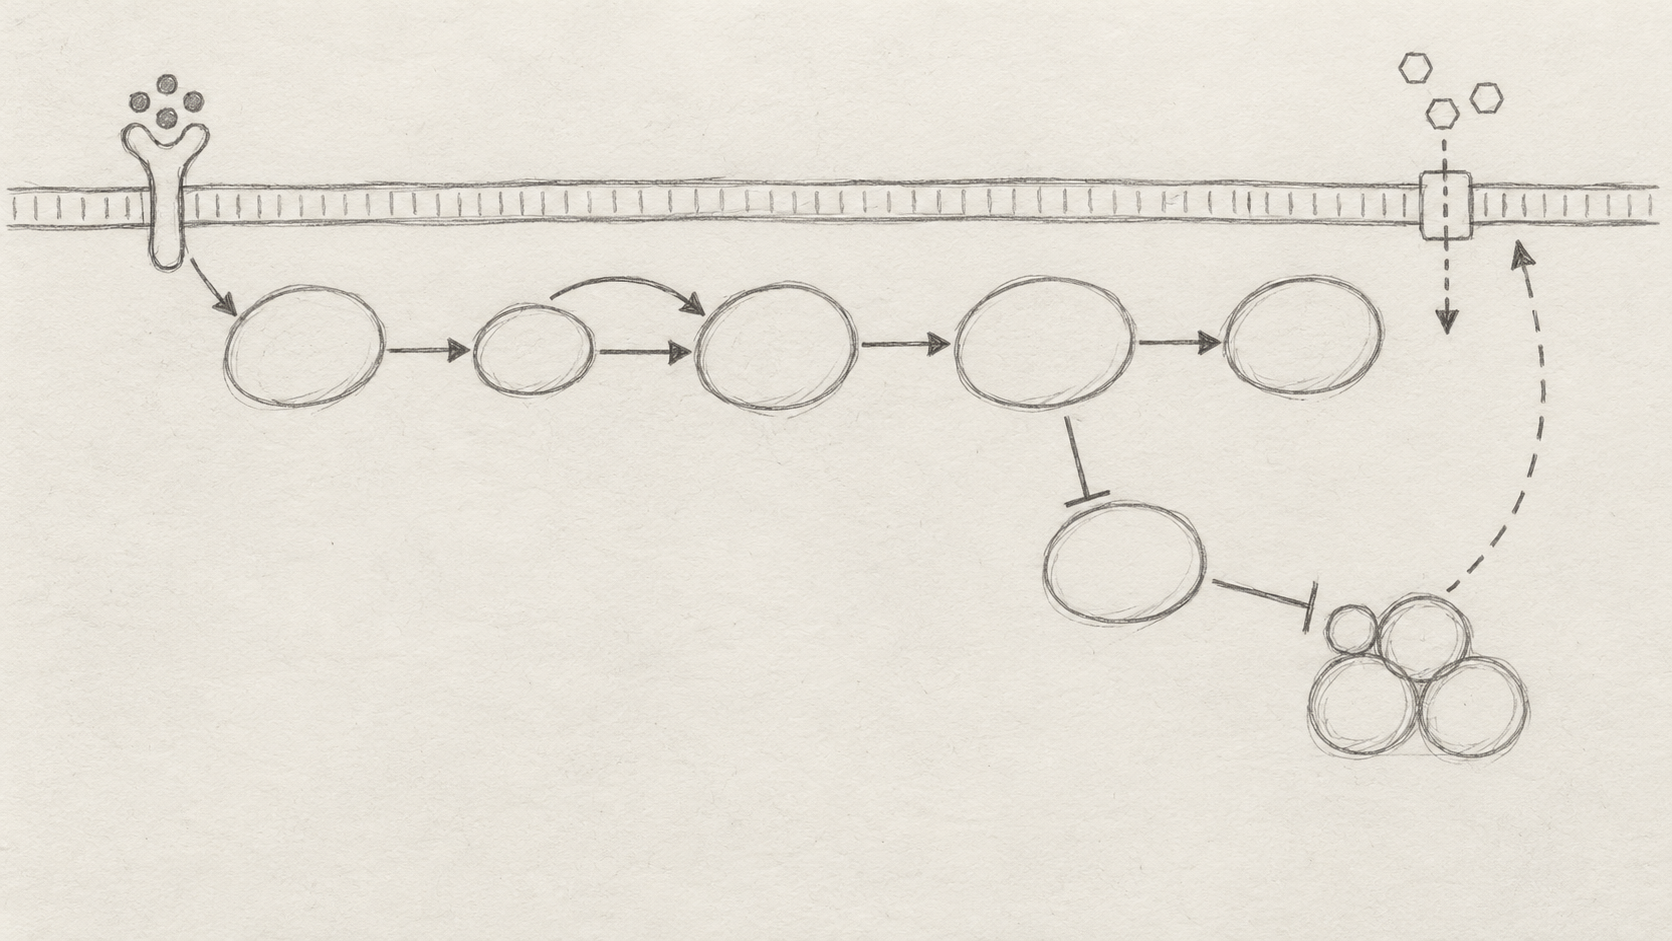
\includegraphics[width=\linewidth]{figures/ch07/ch07-02-v0-sketch.png}};
  \begin{scope}[x={(img.south east)}, y={(img.north west)}]
    \node at (0.12, 1-0.10) {\chsevenrelmark{1}};
    \node at (0.12, 1-0.28) {\chsevenrelmark{2}};
    \node at (0.17, 1-0.44) {\chsevenrelmark{3}};
    \node at (0.25, 1-0.42) {\chsevenrelmark{4}};
    \node at (0.37, 1-0.26) {\chsevenrelmark{5}};
    \node at (0.47, 1-0.37) {\chsevenrelmark{7}};
    \node at (0.53, 1-0.50) {\chsevenrelmark{8}};
    \node at (0.58, 1-0.46) {\chsevenrelmark{9}};
    \node at (0.67, 1-0.58) {\chsevenrelmark{10}};
    \node at (0.80, 1-0.45) {\chsevenrelmark{11}};
    \node at (0.87, 1-0.24) {\chsevenrelmark{12}};
    \node at (0.88, 1-0.12) {\chsevenrelmark{13}};
    \node at (0.44, 1-0.36) {\chsevenrelmark{6}};
  \end{scope}
\end{tikzpicture}
